% revised paper for Energy Journal


\documentclass[11pt]{article}
\usepackage[margin=1in]{geometry}
\usepackage{setspace}
\usepackage{graphicx}
\usepackage{amsmath}
\usepackage{natbib} %for citet and citep
\usepackage{syntonly}
\usepackage{esdiff} %for writing partial derivatives
\usepackage{url} %for inserting urls
\usepackage{placeins} % for limitting floats
\usepackage{comment} %for excluding figures
% \excludecomment{figure} % for printing without figures
% \syntaxonly % for quickly checking document
%set document settings

%\doublespacing % from package setspacs

% table font size
\let\oldtabular\tabular
\renewcommand{\tabular}{\scriptsize\oldtabular}

\title{The Effect of Oil Price on Field Production: Evidence from the Norwegian Continental Shelf}
\author{Johannes Mauritzen\\
		Department of Business and Management Science\\
        NHH Norwegian School of Economics\\
        Helleveien 30, 5045\\
        Bergen, Norway\\
        johannes.mauritzen@nhh.no\\
        \url{jmaurit.github.io}\\
		}
\date{\today}


\begin{document}
 \begin{spacing}{1} %sets spacing to single for title page
	\maketitle


\begin{abstract}
I use detailed field-level data on Norwegian off-shore oil field production and a semi-parametric additive model to control for the production profile of fields to estimate the effect of oil prices on production.  I find no significant evidence of a concurrent reaction of field production to oil prices, though a slight lagged effect is found of the magnitude of approximately 2 to 4\% for a 10 dollar per barrel increase in the real price of oil.  Most of this effect appears to come in the planning phase of a field's development.\\
Keywords: Oil production,Oil Prices, Norway, Semiparametric.
\end{abstract}

\thanks{I would like to thank Klaus Mohn, Jonas Andersson, Sturla Kvamsdal, Harrison Fell, R\"ognvaldur Hannesson and Henrik Horn for valuable discussion and comments.}
% JEL Codes: Q4, L71
 \end{spacing}

\section{Introduction}

For most of the last century, crude oil has been the world’s single most important and valuable fuel source.\footnote{Oil is the world's largest single energy source, consisting of approximately 33\% of total energy consumption in 2013 as well as the most valuable in terms of market price per unit of energy \citep{british_petroleum_statistical_2013}} Naturally, questions of how the oil price affects the world economy as well as how oil production reacts to the oil price have been fundamental topics in economics. 

However a significant gap exists in the literature.  While numerous studies have taken up the issue of how the price of oil affects searching for new fields as well as total oil production at both the regional and global level, few studies exist of the effects of oil prices on oil production at the field level.  The studies that do use field- and well-level data, such as \citet{rao_taxation_2010}, often use data from on-shore installations.  However an increasing amount of the world's oil production comes from hard-to-reach off-shore fields.  Production from challenging off-shore environments is substantially different in character than from on-shore installations.

Moreover, studies within the economics literature fail to take into account how oil prices have varying effects on the different stages of field development and production.  The planning, build-out and depletion phase of a field are conceptually unique and how oil companies operating off-shore respond to oil prices can be expected to vary substantially.

The effect of oil prices on producing fields is an important topic in understanding the mechanisms of how total oil supply reacts in response to price. The response of oil production in existing fields is especially important now as many of the major oil- producing areas, like the Norwegian Continental Shelf are mature and an increasing share of investments will be directed at capacity enhancement in producing fields rather than new field developments. How production from these fields will respond to changes in oil prices has major implications for the oil industry, the state finances of oil-producing countries and long-run oil price formation.

The question of the effect of oil prices on production and the more general question of optimal oil extraction has spawned a large theoretical literature dating back to the seminal work of \citet{hotelling_economics_1931}. \citet{krautkraemer_nonrenewable_1998} provides a good overview. At a basic level a central idea of much of this theoretical work is that with a non-renewable resource, production is a decision that involves a significant opportunity cost: more production in the current period means less production in future periods.  Within this frameworks, prices and expectations of prices become important variables in the production decision. A simple Hotelling model suggests that a producer would immediately change their production in response to a change in oil price in order to dynamically optimize the total extraction.

But in practice, the question is not as clear cut.  Production in the Norwegian Continental Shelf - as well as most other offshore production areas - has extremely high fixed and operating costs.  Keeping spare capacity available in order to adjust to changing oil prices might simply be too expensive.  Instead, producers may find it more beneficial to use storage and financial instruments in order to hedge short-term price movements. Higher oil prices may however still lead a producer to invest in increased capacity.  Since lag times are significant in the off-shore sector, we would then expect to see a multi-year lagged effect of prices on production.  

However even with the question of lagged production and investment, some ambiguity exists.  \citet{mohn_efforts_2008} suggests and finds evidence for the idea that in periods of high oil prices off-shore producers will invest more in risky wild-cat drilling in search of new fields, but concentrate investments in lower-risk ventures, like expanding production in existing fields, when prices are low.  If this effect were to dominate, then it may even be plausible that production in existing fields reacts \emph{negatively} to increases in price. 

%Implications for theories and explanations for understanding of the price mechanism and %the role of speculation.  Hamilton block quote.  

For such a prominent subject, the lack of research on the role of price in oil field production is striking. Two main factors likely contribute to the limited literature - the availability of data and the non-linear time profile of field production.  Large private oil companies, notably the “super majors” and state-owned oil companies have historically accounted for the vast majority of oil production and reserves. \footnote{See for example the economist article titled Supermajordämmerung from August 3rd, 2013: \url{http://www.economist.com/news/briefing/21582522-day-huge-integrated-international-oil-company-drawing}} These entities tend to consider field-level data as either company or state secrets.   

However, over the last few years, a movement towards making the petroleum and other extractive industries more transparent has taken form.  The Norwegian government has been on the forefront of this movement and increasingly committed itself to transparency in the petroleum sector. \footnote{see http://www.regjeringen.no/en/sub/eiti---extractive-industries-tranparency/about-eiti.html?id=633586} Over the last several years, detailed data on most aspects of the country\’s oil industry has become openly available.  

In this article, I use historical production data from all 77 currently or formerly oil-producing fields on the Norwegian continental shelf in order to estimate the effect that prices have on oil production.  

By looking only at the effect of price on fields that currently or previously have produced oil I am limiting the scope of this article.  The effect of oil prices on total production over an extended period of time is due not just to reactions in production in existing fields but also increased searching for new fields.  In fact, an implication of this work is that much of the total production response from higher oil prices is likely from increased searching as well as production from previously un-economic fields.

The main finding in this article is that oil production at the field level has no significant reaction to concurrent changes in the oil price, where concurrent is broadly defined as within the first three years.  A slight effect can be detected at a lag of between 4 and 8 years, with a magnitude of about a 2 to 4\% increase in yearly production for a 10 dollar increase in the price of oil.  This effect is somewhat greater and with less of a lag in large fields compared to small fields.  Price appears to have the most significant affect during the planning stage - before production begins in a field.  In the depletion phase of production, price is found to have little to no significant effect.  

The main methodological problem is the non-linear production profile of oil fields.  Once full-scale extraction is started in an oil field, pressure in wells will start declining. Compensating measures such as gas and water injection have been successful, but their impact is temporary. In turn production rates will therefore inevitably decline.

More so, oil field production is correlated across fields - that is, increases and decreases in production in fields are not randomly distributed across time.  Instead, as figure \ref{top10_production} shows with the production profile of the 10 largest Norwegian oil fields, production tends to be correlated across fields.  The result is a total production curve that is bell-shaped over time as in figure \ref{oil_decline}.  Since the oil price series is autocorrelated and non-stationary, failure to properly account for the production profile will lead to spurious estimation of the price terms in a regression.

The direction of this bias can be gleaned in figure \ref{oil_decline}.  High oil prices were present at periods of relatively low production in the late 1970s and early 1980s as well as over the last 10 years, however real prices reached some of their lowest levels at the same time as the top of production around the year 2000. These oil price dynamics almost certainly affected investment decisions in the industry and in turn total production (\citep{osmundsen_is_2007}, \citep{aune_financial_2010}). However the inverse contemporaneous relationship at the field level is entirely coincidental, but will heavily bias the estimation of the effect of price on production if field production profiles are not properly accounted for. 

\begin{figure}
	\includegraphics[width=1\textwidth]{figures/top10_production_print.png}
	\caption{The production profile of the 10 largest oil fields on the Norwegian Continental Shelf.  Production tends to be correlated across fields}
	\label{top10_production}	
	\end{figure}

\begin{figure}
	\includegraphics[width=1\textwidth]{figures/oil_decline_print.png}
	\caption{The production profile for the entire Norwegian Continental Shelf is bell-shaped, reflecting the correlated production profiles of the fields.  With oil prices that are autocorrelated, }
	\label{oil_decline}
\end{figure}

As a solution I use a semi-parametric model within the Generalized Additive Model frameworks of \cite{hastie_generalized_1990}.  Here I use a two-dimensional smoothed spline function to account for the general non-parametric shape of the production profile while allowing price to enter the equation linearly.  The coefficient of price can then be interpreted as the average effect of price on production over the entire production profile.

\FloatBarrier
\section{The effect of oil price on production: theory, simulations and empirics}

For modeling aggregate oil production, shape-fitting models, notably \citet{hubbert_energy_1962} and more recently advocated by \citet{deffeyes_hubberts_2001}, have had some success in estimating the timing of peak production at the regional and national level, but they tend to seriously underestimate the total recoverable resource of oil-producing regions and the models can be shown to be fundamentally misspecified \citep{boyce_prediction_2013}.   Simulation type studies where aggregate oil production is modeled through an often complex combination of physical and economic processes also exist in the geo-engineering literature, but their usefulness tends to be weighed down by their complexity as they require quite detailed data and specific assumptions about functional form that can be difficult to justify \citet{brandt_review_2010}.

More important to this paper are empirical estimates of the effect of price on production. Several econometric papers seek to answer the question of how aggregated oil supply is affected by oil prices.  \citet{farzin_impact_2001} attempts to estimate an elasticity for the effect on added reserves of increased oil prices and finds a small though statistically significant effect.  \citet{ramcharran_oil_2002} estimates a supply function for the total supply of oil from several OPEC countries based on data from 1973 to 1997.  The author finds a negative price elasticity for several of the countries, and interprets this as evidence of producers targeting revenue.  However since the author does not take into account the production profile of oil fields and the spurious correlation that can arise with autocorrelated prices, these estimates come under considerable doubt.  

the effect of oil-price uncertainty on drilling and exploration has also been explored.  \citet{kellogg_effect_2014} finds that oil exploration firms in Texas do approximately respond as real-option theory would predict when it comes to the timing of drilling.  A model and test using data from North Sea producers on the UK continental shelf by \citet{hurn_geology_1994}, on the other hand, fails to find evidence that the variance in the oil price affects the timing of oil field development.  I do not attempt to directly model uncertainty, however given that the investments needed to increase oil production in an existing field are to a certain extent irreversible and that oil prices are highly volatile, the results can and probably should be interpreted with the real options framework in mind.  

Only a few papers utilize field-level data.  \citet{black_is_1998} tests the relevance of “nesting” a structural empirical model of profit maximization that takes into account oil prices into a typical geo-engineering model of oil field production.  They find strong evidence that taking into account profit maximization, and implicitly price, substantially improves the fit compared to a purely geo-engineering type model.   The limitation of their methodology is that they are only able to test whether including economic factors like price affects the fit of the model but are not able to give an estimate of the effect.  Methodologically, the paper also relies heavily on assumptions about the functional form of both the geo-engineering aspects of the oil producer as well as their profit-maximization.  By taking a more flexible, semi-parametric approach to estimating the effects of oil field production profile, this paper avoids problems with overly restrictive assumptions. 

\citet{rao_taxation_2010} uses data on land based oil wells in California to estimate the effects of tax changes and price controls.  The author finds that short-term tax changes caused small, but significant retiming of production from oil wells.  These findings are over-all consistent with the findings of this paper, though the author finds concurrent effects of taxation on production while I do not find any concurrent effect of prices on production.  This difference is most likely due to the significant differences in cost and complexity between operating offshore and onshore.  How producers react to a short-term tax change as opposed to a change in price is likely also different.  More so, the author does not consider differences between the different stages of production.   

Studies using detailed Norwegian data on offshore activity also exist, though the focus has mainly been on exploration and drilling.  \citet{mohn_exploration_2008} finds that long-term changes in the oil-price has a strong effect on exploratory drilling though little effect is measured from short-term changes in the oil price.  \citet{osmundsen_exploration_2010} analyses drilling productivity over time on the Norwegian Continental Shelf while \citet{mohn_efforts_2008} finds that higher oil prices leads to higher reserves and as well as that oil prices affect producer risk-preferences - with higher prices leading to lower success rates but larger discovery size.  


\section{Oil production on the Norwegian Continental Shelf}


The first commercial oil well in Norwegian continental waters was discovered in December of 1969 in what became the Ekofisk oil field, the largest Norwegian oil field by estimated recoverable reserves.  As figure \ref{north_sea_reserves} shows, most of the largest fields in the North Sea were found relatively early on while more recent finds have tended to be smaller - a pattern typical of oil producing areas called creaming.  A major exception to this trend was the recent find of the Johan Sverdrup field which is estimated to have approximately 300 million Standard Cubic Meters (SM3) of recoverable oil. \footnote{The Johan Sverdrup field is estimated to begin producing oil in 2019 and so is not present in the data set used for the analysis.}  

\begin{figure}
\includegraphics[width=1.2\textwidth]{figures/north_sea_reserves_print.png}
\caption{Oil fields in the Norwegian territorial North Sea.  The largest oil fields tended to be discovered earliest, while newer finds tend to be smaller.  An exception is the large Johan Sverdrup field, which is expected to begin producing in 2019.}
\label{north_sea_reserves}
\end{figure}

Exploration in the Norwegian Sea was opened in the early 1980’s and the first commercial field started production in 1981.  While several mid-sized fields have been discovered, the Norwegian Sea has generally disappointed in terms of commercial oil finds and most finds have been relatively small (\ref{norwegian_sea_reserves}).  

\begin{figure}
\includegraphics[width=1.2\textwidth]{figures/norwegian_sea_reserves_print.png}
\caption{Oil fields in the Norwegian Sea.  Production from the Norwegian Sea has generally been dissapointing compared with expectations when the area was opened to exploration in the early 1980's.}
\label{norwegian_sea_reserves}
\end{figure}

Norwegian waters in the Barents Sea have also been open to exploration since the 1980s, however up until recently only a few, small finds were made and none came into commercial production.  However recently several significant oil and gas finds have been made in the Barents Sea - notably the oil field Goliat and the large gas find Sn\o hvit, which are both currently under development but not yet producing.  The agreement between Norway and Russia in June 2011 settling a long-running dispute over the maritime delimitation has also given a boost to new exploration in the region.  

Profits from oil and gas production in Norway are subject to a resource tax of 50 \% on top of the ordinary income tax of 28 \%, thus income from petroleum production is taxed at a total marginal tax rate of 78 \%.  The central government also receives revenues through ownership stakes in companies, notably Statoil, where the state is the majority stakeholder.  The over-all tax rate has been fairly constant through the history of Norwegian oil production, however several important changes related to the tax code have occurred.  In 1991 a C02 tax was introduced, and in the year 2012 the tax was doubled.  But this was mainly levied on the use and import of petroleum products.  In the offshore sector it was levied on the burning of oil and gas and thus the main effect was on the practice of flaring natural gas that could not be transported and sold commercially.   

More importantly to the offshore sector were accounting changes that were implemented in 2002 and 2005 that were meant to encourage new entrants by allowing losses to be carried forward for tax purposes and by introducing a rebate on the tax-value of losses associated with searching and drilling.  In general though, these rules mainly affected searching and discoveries of new fields rather than production from existing fields and I do not control for the tax changes in my model.  More information on taxation and revenues from the offshore sector can be found at the website of the Norwegian Ministry of Finance. \footnote{\url{http://www.regjeringen.no/en/dep/fin/Selected-topics/taxes-and-duties/bedriftsbeskatning/Taxation-of-petroleum-activities.html?id=417318}}

Rights to explore and eventually produce on the Norwegian Continental Shelf are based on a system where the government announces geographic blocks that will be opened to oil exploration and production subject to production licenses.  Production licenses are initially granted for between 4-6 years subject to requirements that firms are actively searching in their awarded blocks.  If oil or gas deposits are proven then the production license can be extended for up to 30 years.  In general, the frameworks are fair, predictable and stable for companies who find commercially extractable oil deposits and regulatory interference is unlikely to be the cause of any observed changes in production from existing oil fields.  For more information see the website of the Norwegian Petroleum Directorate. \footnote{\url{http://www.npd.no/en/Topics/Production-licences/Theme-articles/Production-licence--licence-to-explore-discover-and-produce-/}}

\section{Norwegian oil field production data}
Production data of Norwegian oil fields is obtained from the website of the Norwegian Petroleum Directorate. \footnote{http://factpages.npd.no/}  Production data is available at a monthly frequency for all fields, though I choose to aggregate up to yearly values both to smooth over seasonality as well as short-term volatility of output due to factors such as weather or technical issues that are not relevant for this article.  

In addition to data on field-level production, I also make use of data on estimated total recoverable reserves. The use of this variable is complicated as it is an estimate subject to a large amount of uncertainty, especially in relatively young fields.  However, the methodologies used to estimate the total recoverable resource of a field are constantly evolving and it is a fair assumption that any consistent bias of the estimates are observed in older fields and corrected for in estimates for newer fields.  I can then assume that existing errors are random and will not significantly bias the estimates.  

Moreover, the estimate is likely endogenous, in the sense that it is also effected by prices.  However since I use the variable as a control variable and not for the purpose of estimating a parameter with a causal interpretation, this should not significantly affect the validity of the results.  

I use yearly data from the US Energy Information Agency on the real price of Brent-traded oil in 2010 dollars.The Brent benchmark oil price is likely the best oil price measure for Norwegian production as it is based on light sweet crude oil sourced from the North Sea.  

An argument can be made that expectations of future oil prices can be equally if not even more important for production decisions as the current oil price.  Forecasts for future oil prices are available from, among others, the International Energy Agency, but these have tended to be notoriously inaccurate and it is unlikely oil companies use these projections for their investment decisions.  

On the other hand, given the size and liquidity of oil spot markets, it is a fair assumption that the current oil prices do a good job of incorporating much of the available information about crude oil markets and that future price movements are generally difficult to predict \citep{hamilton_understanding_2008}.  An active futures market does exist, but several studies have found that current oil prices are in general better than prices on futures contracts at predicting future oil prices \citep{alquist_what_2010, chinn_predictive_2005}.  \citet{mohn_investment_2008} as well as \citet{pesaran_econometric_1990} and \citet{farzin_impact_2001} find evidence for adaptive expectations, where expectations of future prices is based on a weighted average of current and past prices.  I take account of this by including several years of price lags in my regression equations.  

A cleaned data set and the full code for the analysis are available upon request. I use the R statistical programming package for all the analysis in this article \citep{r_core_team_r:_2013}.  I use the R packages ggplot2 and ggmap for plotting \citep{wickham_ggplot2:_2009, kahle_ggmap:_2013}, plyr for data manipulation and cleaning \citep{wickham_split-apply-combine_2011}, texreg for table formatting \citep{leifeld_texreg:_2013} and mgcv for implementation of the Generalized Additive Models \citep{wood_fast_2011}.

\section{A generalized additive model of oil field production}
Parametric linear models have the sizeable advantages of simplicity and interpretability and are therefore usually a good starting point for an analysis.  However, when attempting to model the effect of price on oil field production, a standard linear model is unable to sufficiently control for the production profile and therefore heavily biases the estimate of the effect of price.  As an example, consider a generalized linear model written as in equation \ref{glm_eqn}. 

	\begin{equation}
	\begin{split}	
	 Log(Production_{i,t})  &= \alpha_0 + \alpha_1 timetopeak_{i,t} + \alpha_2 timetopeak_{i,t}^2 \\
	  \quad & + \alpha_3 timetopeak_{i,t}^3  + \alpha_4 peaktoend_{i,t} + \alpha_5 peaktoend_{i,t}^2 \\
	  \quad & + \alpha_6 peaktoend_{i,t}^3 + \gamma totalrecoverableoil_i \\
	  \quad & + \beta_1 oilprice + \beta_2 oilpricel1 + ...+ \beta_6 oilpricel5 + \epsilon	
	\label{glm_eqn}
	\end{split}
	\end{equation}

Here the left hand side variable is yearly production in year $t$ for field $i$.  To try to account for the time profile of production, I split up model-time into a time-to-peak and peak-to-end variable as demonstrated for data for the Statfjord field in figure \ref{statfjord_dem} and then represent each as a cubic function.  Yearly production is assumed to be proportional to the total size of the field as represented by the estimate of the total recoverable resource.  Finally, a term for the oil price as well as five lagged terms are added in order to capture the effects of price.  

\begin{figure}
\includegraphics[width=1\textwidth]{figures/statfjord_dem_print.png}
\caption{The production profile can be modeled in two phases - time-to-peak, representing the build-out phase of the oil field and time-from-peak, representing the period of depletion. The is illustrated with data from the Statfjord field.}
\label{statfjord_dem}
\end{figure}

Figure \ref{glm_dirty_box} shows the estimates of the coefficients on the oil price and its lags \footnote{The dots on the figure represent 1000 simulations of the estimated coefficient based on the estimated standard error and point estimate from the model}.  The lags are not estimated to have an effect significantly different from zero. However a literal interpretation of the coefficient on the concurrent oil price term would indicate that a 10-dollar increase in the oil price would lead to a lowering of field production of around 4-5\%.

\begin{figure}
\includegraphics[width=1\textwidth]{figures/glm_dirty_box_print.png}
\caption{A generalized linear model generates a negative estimate of the coefficient on price in a regression on production.  This result is spurious, caused by a failure to properly control for the production profiles of the fields.}
\label{glm_dirty_box}
\end{figure}

This estimate is heavily biased downwards due to the spurious correlation between the field production profiles and the autocorrelated and non-stationary time series of oil prices.  A more formal analysis of the bias can be found in Appendix B, where I simulate data of oil field production in a Monte Carlo experiment.  However, the basic idea is that the parametric representation is not flexible enough to control for the production profiles of the fields.   Instead, a more flexible estimation of the production profile is needed. 

Instead of attempting to estimate the shape of the production profiles of the fields by estimating parameters on linear terms I estimate a non-parametric function for the production profile.  As an illustration, consider the production profile of a single field.  The simplest possible model would then have the form of equation \ref{simp_eqn}. 

\begin{equation}
Production_{t}=f(time) + \epsilon
	\label{simp_eqn}
\end{equation}

Again considering the production profile for the Statfjord field, a smoothed function might look like the black line in figure \ref{statfjord_gam}.   

\begin{figure}
	\includegraphics[width=1\textwidth]{figures/statfjord_gam_print.png}
	\caption{An illustration of fitting a simple non-parametric function to the production profile of a single field.}
	\label{statfjord_gam}
\end{figure}

In principle any number of well-behaved smoothers could be used to estimate the function, for example a Loess or a kernel smoother.  In practice regression splines are most commonly used.  With a regression spline the data points for the function to be estimated are broken into bins.  For each bin of data a local linear regression is estimated.  For functions of one variable, a cubic parameterization is often used.  These regressions are then essentially tied together at what are called “knots” and the smoothness of the overall function is controlled by a penalty function that consists of the second derivative of the estimated function.

In my regression, I find it helpful to represent the production profile of fields as a two-dimensional function.  This can not be accomplished with a standard cubic regression spline, but I can instead use a Thin Plate (Regression) Spline \citep{wood_thin_2003}.  Though the full details of the implementation are beyond the scope of this paper, for the basic idea consider equation \ref{thin_plate_1}.  

	\begin{equation}
	y_i = g(x_1, x_2)
	\label{thin_plate_1}
	\end{equation}

Following \citet{wood_generalized_2006}, $g$ is the function of $x_1$ and $x_2$ that is to be estimated by $f$, which in turn is estimated by minimizing equation \ref{thin_plate_2}.  Here $\boldsymbol{y}$ represents a vector of $y_i$’s and $\boldsymbol{f} = (f(\boldsymbol{x_1}),f(\boldsymbol{x_2}))^t$.   

	\begin{equation}
\min \|\boldsymbol{y-f}\|^2 + \lambda J_{22}(f)
\label{thin_plate_2}
	\end{equation}

$J_{22}$ represents the penalty function for the smoothness of the function which can be written as in \ref{thin_plate_3}.  The $22$ represents the fact that it is a penalty function of two variables with smoothness measured by the second derivative.

	\begin{equation}
	J_{22}{f}= \diffp[2]{f}{x_1}^2 + \diffp[2]{f}{{x_1}{x_2}} + \diffp[2]{f}{x_2}^2dx_1 dx_2
\label{thin_plate_3}
	\end{equation}

In short, a function of $x_1$ and $x_2$ is found that is minimizing errors in the sense of minimizing Euclidean distance subject to a penalty function of “wiggiliness”.  The actual implementation is somewhat more involved in order to increase the computational efficiency of the estimation.  For further details I again refer to \citet{wood_thin_2003}.

The advantage to using splines over other smoothing methods is that it can be represented in a linear form.  Thus estimation of the model can be done using standard and efficient matrix algebra algorithms. For further details I refer to the discussion in \citet{hastie_generalized_1990} and \citet{wood_generalized_2006}.  The latter is a particularly useful reference for implementing generalized additive models in R.

I do not want to estimate smoothed curves individually for each field.  While this would provide a good overall fit to the full data set, not enough variation in the data would be left to estimate the effect of price.  Instead I want to estimate a general shape of the production profile for all fields and then use the remaining variation in the data to estimate the effect of price.  My model can be written as in equations \ref{gam_price_eqn}.

\begin{equation}
\begin{split}

	Log(Production_{i,t}) & = f(time\_to\_peak_{i,t}, total\_recoverable\_oil_i) \\
 	 \quad & + f(peak\_to\_end_{i,t}, total\_recoverable\_oil_i) \\
	 \quad & + \beta_1 oil\_price + \beta_2 oil\_price\_l1 + ... +  \epsilon
\label{gam_price_eqn}
\end{split}
\end{equation}

In this model I am estimating the parameters and functions from all fields $i$. As in the parametric model presented earlier, the left-hand-side variable is yearly oil production for field $i$. Also like the parametric model I split the production-time component element in two: up to and after the peak in production. 
While a shape for the entire production profile could be estimated with one smoothed function, splitting it up allows for more flexibility and better overall fit of the model as estimated by deviance score and the related estimated degrees of freedom of the model.  More so, production up to a peak and the subsequent decline represents two distinct processes.  The first is driven by the physical investment and build-out of the field, while the latter is dominated by depletion of the field and subsequent drop in pressure. It makes sense to model these two processes separately, and later I will also attempt to estimate separate price effects for the two phases. 

I also allow the smoothed functions to vary with the total size of the field as measured by the estimated total recoverable oil since the shape of the production profile tends to vary substantially by field size.  Inspection of a selection of fields, such as shown in figure \ref{field_inspection}, shows that smaller fields tend to reach their peak quickly while larger fields take more time. 

The estimated field-size variable is however an imperfect measure.  First, estimates for newer fields will likely have higher measurement errors than established fields that are well explored and where a significant amount of the oil has already been extracted.  The total reserves estimates are also likely correlated with the price terms as estimates of recoverable reserves likely change depending on the level of the oil price.  Nonetheless, since I am only using the variable to help to control for the general shape of the production profiles of fields and not as an exogenous regressor, the inclusion of the variable should not materially affect the estimation.

\begin{figure}
	\includegraphics[width=1\textwidth]{figures/field_inspection_print.png}
	\caption{A selection of production profiles of oil fields.  The shape can vary substantially by field size as well as other factors.}
	\label{field_inspection}
\end{figure}

Even with a smoothed function that is allowed to vary by field-size, a substantially better fit, as well as more nuanced analysis could be obtained by splitting the estimation into small and large fields, this time measured by the maximum production of the field - a measure of field size that is less likely to be highly correlated with price.  The improvement in fit can be seen by inspecting the fitted values of the models as in figure \ref{bench_vs_split}. The split estimation provides a particularly better fit for smaller and mid-sized fields.

\begin{figure}
	\includegraphics[width=1\textwidth]{figures/bench_vs_split_print.png}
	\caption{A benchmarking model shows that a substantially better fit can be achieved by splitting the analysis into small and large fields, where a somewhat arbitrary maximum yearly production of 8 million SMU is used as the separating value.}
	\label{bench_vs_split}
\end{figure}

Plots of the estimated smoothed functions in the model are not directly informative about the effects of price and so I do not include them in the main text.  However they can be helpful in gaining a intuition behind the estimation procedure so I have included them in appendix 2 along with other model diagnostics and robustness checks.  

\section{The Effect of Oil Price on Field Production}

The variables of interest in this article is the oil price and its lags, which I include as nine linear parametric terms in the model.  The idea of including both a concurrent oil price term as well as eight lags is that a change in price could conceivably have two effects on oil production in a field.  First, the field operator could be operating on the basis of some short-term extraction rule - choosing to pump out less at times of lower prices in order to pump out more at periods of high prices.  

Alternatively, a change in price of oil can be seen as a lifting of a production constraint.  A higher oil price means that added investments in production become attractive in order to either increase the total amount extracted from a field or to shift production forward.  However investments in the offshore sector can be complex and lengthy, and any production lift would be expected to happen with a lag.  As mentioned earlier, including several lags also allows for the possibility of adaptive expectations of future oil prices.The results for the price terms are shown in figure \ref{gam_price_8}.

\begin{figure}
	\includegraphics[width=1\textwidth]{figures/gam_price_8_print.png}
	\caption{The coefficient estimates on the price terms where two additional lags are added to the model.  Significant positive results are found on the 8th lag for both large and small fields, providing evidence for adaptive price expectations by producers.}
	\label{gam_price_8}
\end{figure}
 

The estimated coefficients for the concurrent and first three lags of the oil price are not estimated to be significantly different than zero.  For large fields a modest effect at the fourth, sixth and seventh lags are estimated, though only at a 10\% significance level, \footnote{The lines in the boxplot represent conservative 95\% confidence intervals and are calculated using a bayesian-inspired simulation from the posterior distribution of the coefficients.  P-values (stars) shown in the table in the appendix were calculated by standard asymptotic methods and show significant results for the 4th and 6th lags at the 5\% level.} while for small fields an effect is estimated only at the sixth lags. The magnitude of these effects is in the neighborhood of a 2\% increase in production for a 10 dollar increase in the oil price.  A larger and more significant effect is found for both small and large fields at the 8th lag, with a magnitude implying an approximately 3 to 4\% increase in production for a 10 dollar increase in the oil price.  

Despite the clear implications of most simplified Hotelling models, the lack of significant results for the concurrent price and the modest lagged effect is not surprising. In general, operating an oil production rig and related offshore infrastructure is an extremely expensive venture with high fixed costs.  In the challenging conditions of the North Sea, the expenses are multiplied.  Thus any short-term benefit of strategically altering production in relation to movements in the oil price are dominated by the large costs of having excess pumping capacity.  In other words, oil producers have a strong incentive to pump as much oil out at any given time given the existing production capacity.

Instead, the results point to a mechanism where oil producers react to higher oil prices by increasing investment in those fields, leading to higher oil production only with a considerable lag.   This story is in line with a trend of increased total extraction estimates from the Norwegian continental shelf as a whole as well as from existing fields over the last 15 years of strongly rising oil prices \footnote{\url{http://npd.no/Templates/OD/Article.aspx?id=4731&epslanguage=en}}.

I prefer the un-pooled models I have presented above because of the improvement in model fit and because operators of small and large fields may be expected to have substantially different reactions to changes in price as well as different time profiles of production. Nonetheless, it can be instructive to show results from a pooled model where a fixed effect and interaction variable is introduced to distinguish the effects of small and large fields. The model can be written as equation \ref{pooled_eqn}.  The terms in the model are mostly the same as in \ref{gam_price_eqn} but with an added dummy term for small fields - those with a maximum yearly production of 8 million SM3 or below, $smallfield$, and interaction terms.  

\begin{equation}
\begin{split}
	Log(Production_{i,t})&=f(timetopeak_{i,t}, totalrecoverableoil_i) \\
	 \quad & + f(peaktoend_{i,t}, totalrecoverableoil_i) \\
	 \quad & + \beta_1 oilprice + \beta_2 oilpricel1 + \dots + oilpricel8\\
	 \quad & + \delta smallfield \\
 	 \quad & + \gamma_1 oilprice*smallfield + \gamma_2 oilprice*smallfield + \dots \\
 	 \quad & + oilpricel8*smallfield +  \epsilon
\label{pooled_eqn}
\end{split}
\end{equation}

The full results for the estimates of all the parametric terms can be found in table \ref{table:pooled} in the appendix.  The estimated coefficients on the price terms are shown in figure \ref{gam_price_pooled}. In the regression none of the interaction effects were significantly different than zero, nor were the concurrent price term or the first three lags.  The fourth and sixth through eighth lag were however significant and positive, again at a magnitude of approximately 2\% increase in production for a \$10 increase in the oil price.

\begin{figure}
	\includegraphics[width=1\textwidth]{figures/gam_price_pooled_print.png}
	\caption{The estimated coefficients on the price terms for a pooled model of oil field production.  Significant estimates are found on the fourth, sixth, seventh and eighth price lags}
	\label{gam_price_pooled}
\end{figure}

In the above discussion, I have been implicitly giving the coefficients a causal interpretation, which deserves some discussion.  My main identifying assumption is that production at the field level can not cause significant changes in the oil price.  A stronger but still relevant assumption that may be necessary since field production is correlated across fields is that total production from the Norwegian continental shelf does not affect oil price.  

Both of these assumptions are likely satisfied.  Oil is a globally traded commodity and total Norwegian production accounts only for a small fraction of total production.  In 2013 Norwegian production made up only 2.3 \% of the world total. \footnote{\url{http://www.eia.gov/countries/country-data.cfm?fips=NO#pet}}  A drastic change in production, on par with the halt in production that occurred in Libya in 2011, \footnote{Before the Libyan revolution of 2011, Norwegian and Libyan yearly oil production were of a similar magnitude, 2.1 versus 1.8 million barrels of oil in 2010 \url{http://www.eia.gov/countries/country-data.cfm?fips=LY#pet}} would have been required to have had any significant effect on world oil supply and in turn prices. 

One of the main implications of the interpretation that higher oil prices leads to increased extraction through increased investment is that while the effect on production will be lagged, higher oil prices will have a more immediate effect on investments.  I test for this with the model as written in equation \ref{gam_invest_eqn}

\begin{equation}
\begin{split}
	Log(Investment_{i,t})&=f(timetopeak_{i,t}, totalrecoverableoil_i) \\
	 \quad &+ f(peaktoend_{i,t}, totalrecoverableoil_i) \\
	 \quad &+ \alpha oilproduction_{i,t} \\
	 \quad & + \beta_1 oilprice + \beta_2 oilpricel1 + ... + oil_pricel8 \\
	 \quad &+ \delta smallfield \\
	 \quad &+ \gamma_1 oilprice*smallfield + \gamma_2 oilprice*smallfield + ... 
	+  \epsilon \\
\label{gam_invest_eqn}
\end{split}
\end{equation}

In the equation investment in each field $i$ at time $t$ is a function of the state of field development, as modeled by a non-parametric function of time to and from the peak as well as the total size of the field - as in the model of oil field production.  In addition I include a term for oil production in field $i$ at time $t$.  The coefficients of interest are again those on the oil price and its lags which I interact with a dummy variable for large and small fields, $smallfield$.

The results for the estimation of the estimated coefficients on the oil price and its lags is shown in figure \ref{gam_price_invest_box} while full results are also shown in table \ref{table:investment} in appendix 1.  The coefficient on the concurrent oil price as well as the third and fourth lags are all significantly positive, with coefficients that can be interpreted to mean that a 10 dollar increase in the oil price leads to between a 5 to 10 \% increase in oil field investment in the concurrent and second subsequent year and between a 10 to 20\% increase in the third subsequent year.  

\begin{figure}
	\includegraphics[width=1\textwidth]{figures/invest_pooled_print.png}
	\caption{Estimated coefficients for the price terms in a model of oil field investments.  A rise in the oil price leads to an increase in investment in the concurrent year as well as in the second and third lag. Negative coefficients are found for the sixth through 8th lags.}
	\label{gam_price_invest_box}
\end{figure}

The results of the regression on investment fits nicely with the previous results on oil production which showed a significant effect in the 4th through 6th lags.  A story consistent with both results is that higher oil prices induce increased investment in production capacity, though it takes time to get the extra capacity in place and the effects on production to be felt.

The estimated coefficients on the 6th, 7th and 8th lagged coefficients are shown to be significantly negative. An explanation is that a higher oil price induces producers to speed up a build out of a field, leading to more investment earlier, but relatively less in later years.  An implication of this theory is that the effect of price will primarily be in the build-out phase of a fields production profile.  This is explored in the following section.

\section{The effect of price in the phases of oil production}

Treating the entire production life of an oil field as essentially the same process is an oversimplification of the industry and field dynamics.  A field's life can be split into roughly three periods.  Before physical investment and production can begin, an often times lengthy planning stage occurs.  In this stage, the extent and details of a fields build-out are decided and must receive approval from the Norwegian Petroleum Directorate as well as other government agencies.  

Once plans have been approved and finalized, the build-out phase of a field can begin.  The field operator has an incentive to build out the field as quickly as possible as large amounts of capital have at that point been allocated and it is important to get oil production and in turn income flowing as quickly as possible.  Once the build-out is complete and production has reached its peak, geophysical forces that come from depletion and subsequent drop in field pressure dominate.  Here technological change can also play a role - with improvements over time - like the introduction of gas and water injection - allowing for increased recovery percentage of the available reservoir. 

In the preceding sections I have partially taken account of the different dynamics of the phases of field production by modeling post- and pre-peak production as seperate smoothed terms.  However, the price variable was estimated for the entire production profile.  The advantage of this approach is that I am able to use the full data-set and estimate a total average effect.  However the effect of price can reasonably be expected to differ in the different phases of production.  

In this section I model the pre-peak and post-peak periods of production separately - including the price terms. The vast majority of producing fields in Norway are well past their peak production and because larger fields tended to be found earlier, an even larger share of total oil production comes from depleting fields.  In terms of policy implications, the most important question is what the effect of price has on post-peak production. 

To ensure that no fields are included in the post-peak group that have not been fully built-out yet and which have not reached their peak production, I exclude all fields that began oil production prior to 2008.  While some large fields may take slightly more than five years to fully build out, none such fields began production in that time frame.

 The estimated coefficients on the price term for post-peak production is shown in figure \ref{gam_postpeak_print}.  The full results are shown in table \ref{table:postpeak} in the appendix.  The results mostly show no significant effect of price on production through the 7th lag, though positive coefficients for large fields are estimated for all but the 5th lag.  

 A significant positive coefficient is estimated on the first lag for small fields, however this result is not robust to specification.  Using the maximum production instead of estimated total oil reserves in the smoothed function gives a somewhat better fit for some small fields (see figure \ref{chart:Max_prod_vs_TRO_print} in Appendex 2).  In this regression the coefficient is estiamted to be smaller and is no longer significant (see table \ref{table:postpeak}).  When small and large fields are pooled in one regression, this coefficient is again not estimated to be significantly different from zero.  This estimated coefficient should be met with some skepticism.  

 On the other hand, the significant coefficient on the 8th lag for small fields is robust to specification. From an industry perspective, why price should have a 8-year-lagged effect on small fields but not large fields may not be immediately clear, but the length of the lag combined with the relatively short life of small fields suggests that the effect of price occurs well before the depletion phase begins.  

\begin{figure}
	\includegraphics[width=1\textwidth]{figures/gam_postpeak_print.png}
	\caption{The estimated coefficients on the price terms in a model of oil field production in depleting fields.  Significant coefficients are only estimated on the concurrent price and eight lag, however the significance of the estimated coefficient on the eighth lag is not robust to specification}
	\label{gam_postpeak_print}
\end{figure}

The effect that price has on production from a declining fields appears to be, at best, slight.  The point estimates on the price terms for large fields are of a magnitude of around 1\% - 2\% for a 10 dollar increase in the price of oil, but as noted, these estimates are not significantly different from zero.  In general, no clear relationship appears in the data between production and prices.

However, to say that price has no effect on production from depleting fields may be too strong. One mechanism for prices to effect production in depleting oil fields that this regression may not directly capture is through technological change.  Higher prices may encourage more research and development and in turn lead to innovations that increase the total recovery percentage of a field.  For example, over the course of the history of Norwegian oil production, innovations such as horizontal drilling and four-dimensional geological visualization have led to increased estimates of the total recovery rate of Norwegian oil fields.  However, this mechanism is likely too diffuse - lacking any consistent relationship between price, innovation and subsequent increases in production - to be captured by the regressions in this analysis. 

While price appears to have little affect on production in depleting fields, it may have an effect in the planning and build-out phase of production. I run a regression model of field production up to peak production, representing the build-out phase of a field.  Because of the double-peak profile of the Ekofisk field, I only include data from this field up to the initial peak in 1976.  The full results can be found in table \ref{table:prepeak} in Appendix I.  I show the estimated coefficient on the price terms in table \ref{gam_prepeak_print} below.  

\begin{figure}
	\includegraphics[width=1\textwidth]{figures/gam_prepeak_print.png}
	\caption{The estimated coefficients on the price terms in a model of fields in the build-out phase.  For large fields, positive coefficients are estimated at the 6th, 7th and 8th lag, but the estimates are imprecise and not statistically significant.  Significant positive coefficients are estimated for small fields at the fifth and eighth lag.  In a pooled model, significant positive coefficients are found at the fourth through eighth lags.}
	\label{gam_prepeak_print}
\end{figure}

What is immediately noticeably is the imprecision of the price estimates in the model of the large fields.  This is primarily due to a lack of data points.  The estimates are based on only 76 data points from 11 fields.  Positive coefficients are estimated at the 6th, 7th and 8th lag, though none of these are statistically significant at the 95\% level.  The coefficient on the lagged price terms for small fields, however, are estimated to be positive and significant at the 5th and 8th lags.  

I also estimate a pooled model, with both small and large fields.  This model provides a worse overall fit than the split model, but can nonetheless be useful given the few data points available for large fields.  The coefficients on the 1st as well as 3rd to through 8th lags are all estimated to be significant and positive at a magnitude that corresponds to approximately 2-8 \% increase in oil production for a 10 dollar increase in the cost of a barrel of oil.

\begin{figure}
	\includegraphics[width=1\textwidth]{figures/field_time_to_peak_print.png}
	\caption{A histogram of the number of year before a field is fully built out and a field reaches its peak production.  The vast majority of fields, especially small fields, are built out quickly - within one or two years.}
	\label{gam_buildout_hist}
\end{figure}

Figure \ref{gam_buildout_hist} shows a histogram of the time it takes to fully build out an oil field and reach peak production.  We see that the vast majority of fields are built out quickly, reaching their peak production within one or two years.  Since the effect of price on the build-out phase is estimated with a lag of between 5 and 8 year, this indicates that changes in price likely has most effect well before production in a field even begins.  In turn, this suggests that changes in price that occur during the planning stage of a fields development are the most important in determining the production of the field.  This result fits well with the industry structure.  As mentioned, before physical investment in a field can begin and production started, detailed plans need to be approved by several government agencies and capital must be allocated.  Changing the level of investments in reaction to a change in prices after plans have been finalized is likely to lead to both an expensive delay as well as other costs that heavily outweigh any benefits of increased future production.  




\section{Conclusion}

The main results of this research is to show that production in existing Norwegian offshore fields has no significant concurrent reaction to higher oil prices while a slight effect is estimated  with a lag of between 4 and 8 years.  Oil producers do not appear to be behaving strategically in relation to short-term production - increasing or reducing production in response to changes in oil price.  Instead they are likely using storage or financial instruments to hedge short-term price movements. Changes in oil prices can rather be seen as a relaxing of a production constraint, justifying increased investment that leads to either a higher total extraction rate or an inter-temporal shifting of production. Furthermore, it appears that the most of the effect of price comes at the planning phase of a field's production life.  Little to no effect of price on production is found in the build-out or depletion phase.

The modest estimated effect of prices on production adds weight to the argument of \citet{hamilton_oil_2012} that most of the increased supply of oil that comes from higher prices is from expanding the geographic and technological boundaries of oil production.  For example exploration of deep-water oil deposits off the coast of Brazil and extraction of oil sands in western Canada.   

 \begin{spacing}{1}

\bibliographystyle{plainnat}
\bibliography{oil_prices}

% \end{spacing}
% \end{document} for shorter version with no appendix
\FloatBarrier

\appendix

\section{Appendix: Tables of full results and robustness checks}

\begin{table}
\begin{center}
\begin{tabular}{l c c c c c c }
\hline
	&\multicolumn{2}{|c|}{6 lags} & \multicolumn{2}{c}{8 lags} &\multicolumn{2}{c}{4-8 lags} \\
                                     & Small & Large & Small  & Large & Small & Large\\
\hline
(Intercept)                          & $-1.46^{***}$ & $-0.15$       & $-1.58^{***}$ & $-0.25$       & $-1.54^{***}$ & $-1.54^{***}$ \\
                                     & $(0.37)$      & $(0.50)$      & $(0.38)$      & $(0.51)$      & $(0.37)$      & $(0.37)$      \\
oilpricereal                       & $0.00$        & $-0.02$       & $0.00$        & $-0.01$       &               &               \\
                                     & $(0.01)$      & $(0.01)$      & $(0.01)$      & $(0.01)$      &               &               \\
oilpricereall1                    & $0.01$        & $-0.01$       & $0.01$        & $0.01$        &               &               \\
                                     & $(0.01)$      & $(0.01)$      & $(0.01)$      & $(0.01)$      &               &               \\
oilpricereall2                    & $-0.02$       & $0.01$        & $-0.01$       & $0.00$        &               &               \\
                                     & $(0.01)$      & $(0.01)$      & $(0.01)$      & $(0.01)$      &               &               \\
oilpricereall3                    & $-0.02$       & $0.01$        & $-0.03^{*}$   & $0.00$        &               &               \\
                                     & $(0.01)$      & $(0.01)$      & $(0.01)$      & $(0.01)$      &               &               \\
oilpricereall4                    & $0.00$        & $0.03^{*}$    & $0.00$        & $0.03^{*}$    & $-0.01$       & $-0.01$       \\
                                     & $(0.01)$      & $(0.01)$      & $(0.01)$      & $(0.01)$      & $(0.01)$      & $(0.01)$      \\
oilpricereall5                    & $-0.01$       & $0.01$        & $-0.01$       & $0.01$        & $-0.02$       & $-0.02$       \\
                                     & $(0.01)$      & $(0.01)$      & $(0.01)$      & $(0.01)$      & $(0.01)$      & $(0.01)$      \\
oilpricereall6                    & $0.02^{*}$    & $0.03^{*}$    & $0.02$        & $0.01$        & $0.02^{*}$    & $0.02^{*}$    \\
                                     & $(0.01)$      & $(0.01)$      & $(0.01)$      & $(0.01)$      & $(0.01)$      & $(0.01)$      \\
EDF: s(timetopeak,recoverableoil) & $28.92^{***}$ & $26.89^{***}$ & $28.91^{***}$ & $26.89^{***}$ & $28.91^{***}$ & $28.91^{***}$ \\
                                     & $(29.00)$     & $(27.00)$     & $(29.00)$     & $(27.00)$     & $(29.00)$     & $(29.00)$     \\
EDF: s(peaktoend,recoverableoil)  & $17.75^{***}$ & $10.71^{***}$ & $17.58^{***}$ & $11.41^{***}$ & $17.47^{***}$ & $17.47^{***}$ \\
                                     & $(28.00)$     & $(28.00)$     & $(28.00)$     & $(28.00)$     & $(28.00)$     & $(28.00)$     \\
oilpricereall7                    &               &               & $-0.01$       & $0.02^{*}$    & $-0.01$       & $-0.01$       \\
                                     &               &               & $(0.01)$      & $(0.01)$      & $(0.01)$      & $(0.01)$      \\
oilpricereall8                    &               &               & $0.04^{***}$  & $0.03^{**}$   & $0.03^{***}$  & $0.03^{***}$  \\
                                     &               &               & $(0.01)$      & $(0.01)$      & $(0.01)$      & $(0.01)$      \\
\hline
AIC                                  &               & 1211.33       &               & 1186.97       &               &               \\
BIC                                  &               & 1377.97       &               & 1363.28       &               &               \\
Log Likelihood                       &               & -559.07       &               & -544.18       &               &               \\
Deviance                             & 12319.62      & 301090.57     & 12104.52      & 268975.69     & 12347.62      & 12347.62      \\
Deviance explained                   & 0.84          & 0.96          & 0.85          & 0.96          & 0.84          & 0.84          \\
Dispersion                           & 15.17         & 1378.61       & 14.93         & 1247.02       & 15.16         & 15.16         \\
R$^2$                                & 0.82          & 0.95          & 0.83          & 0.95          & 0.82          & 0.82          \\
GCV score                            & 16.19         & 1666.44       & 15.98         & 1526.28       & 16.13         & 16.13         \\
Num. obs.                            & 865           & 264           & 865           & 264           & 865           & 865           \\
Num. smooth terms                    & 2             & 2             & 2             & 2             & 2             & 2             \\
\hline
\multicolumn{7}{l}{\scriptsize{\textsuperscript{***}$p<0.001$, 
  \textsuperscript{**}$p<0.01$, 
  \textsuperscript{*}$p<0.05$}}
\end{tabular}
\caption{Full results for model of field production with price, seperate estimation of small and large fields.}
\label{table:unpooled}
\end{center}
\end{table}



%table two pooled
\begin{table}
\begin{center}
\begin{tabular}{l c c }
\hline
                                     & Pooled Model & Insignificant terms dropped \\
\hline
(Intercept)                          & $-1465.35^{***}$ & $-1500.51^{***}$ \\
                                     & $(65.21)$        & $(66.28)$        \\
oilpricereal                       & $-0.01$          &                  \\
                                     & $(0.01)$         &                  \\
largefieldsmall                     & $-2.32^{***}$    & $-1.19^{***}$    \\
                                     & $(0.27)$         & $(0.10)$         \\
oilpricereall1                    & $0.02^{*}$       &                  \\
                                     & $(0.01)$         &                  \\
oilpricereall2                    & $0.01$           &                  \\
                                     & $(0.01)$         &                  \\
oilpricereall3                    & $0.00$           &                  \\
                                     & $(0.01)$         &                  \\
oilpricereall4                    & $0.03^{***}$     & $0.03^{***}$     \\
                                     & $(0.01)$         & $(0.01)$         \\
oilpricereall5                    & $0.01$           & $0.01$           \\
                                     & $(0.01)$         & $(0.01)$         \\
oilpricereall6                    & $0.02^{***}$     & $0.03^{***}$     \\
                                     & $(0.01)$         & $(0.01)$         \\
oilpricereall7                    & $0.02^{**}$      & $0.02^{***}$     \\
                                     & $(0.01)$         & $(0.01)$         \\
oilpricereall8                    & $0.03^{***}$     & $0.03^{***}$     \\
                                     & $(0.00)$         & $(0.00)$         \\
oilpricereal:largefieldsmall      & $-0.03$          &                  \\
                                     & $(0.06)$         &                  \\
largefieldsmall:oilpricereall1   & $0.03$           &                  \\
                                     & $(0.07)$         &                  \\
largefieldsmall:oilpricereall2   & $-0.05$          &                  \\
                                     & $(0.08)$         &                  \\
largefieldsmall:oilpricereall3   & $0.03$           &                  \\
                                     & $(0.07)$         &                  \\
largefieldsmall:oilpricereall4   & $0.03$           &                  \\
                                     & $(0.07)$         &                  \\
largefieldsmall:oilpricereall5   & $0.04$           &                  \\
                                     & $(0.07)$         &                  \\
largefieldsmall:oilpricereall6   & $0.18^{*}$       &                  \\
                                     & $(0.07)$         &                  \\
largefieldsmall:oilpricereall7   & $0.06$           &                  \\
                                     & $(0.07)$         &                  \\
largefieldsmall:oilpricereall8   & $0.07$           &                  \\
                                     & $(0.07)$         &                  \\
EDF: s(timetopeak,recoverableoil) & $28.99^{***}$    & $28.99^{***}$    \\
                                     & $(29.00)$        & $(29.00)$        \\
EDF: s(peaktoend,recoverableoil)  & $27.98^{***}$    & $26.99^{***}$    \\
                                     & $(28.00)$        & $(27.00)$        \\
\hline
AIC                                  &                  &                  \\
BIC                                  &                  &                  \\
Log Likelihood                       &                  &                  \\
Deviance                             & 371079.07        & 396494.49        \\
Deviance explained                   & 0.96             & 0.96             \\
Dispersion                           & 352.06           & 371.24           \\
R$^2$                                & 0.96             & 0.95             \\
GCV score                            & 377.77           & 393.13           \\
Num. obs.                            & 1129             & 1129             \\
Num. smooth terms                    & 2                & 2                \\
\hline
\multicolumn{3}{l}{\scriptsize{\textsuperscript{***}$p<0.001$, 
  \textsuperscript{**}$p<0.01$, 
  \textsuperscript{*}$p<0.05$}}
\end{tabular}
\caption{Full results for pooled model of field production with price terms.}
\label{table:pooled}
\end{center}
\end{table} 


%investment tables

\begin{table}
\begin{center}
\begin{tabular}{l c c c }
\hline
                                     & Pooled & Small Fields & Large Fields \\
\hline
(Intercept)                          & $-199.84^{***}$ & $7.03^{***}$   & $7.64^{***}$    \\
                                     & $(44.00)$       & $(0.36)$       & $(0.24)$        \\
yearprod                            & $-0.06^{***}$   & $-0.26^{***}$  & $-0.06^{***}$   \\
                                     & $(0.01)$        & $(0.02)$       & $(0.01)$        \\
oilpricereal                       & $0.08^{***}$    & $-0.03^{**}$   & $0.04$          \\
                                     & $(0.01)$        & $(0.01)$       & $(0.03)$        \\
largefieldsmall                     & $1.80^{***}$    &                &                 \\
                                     & $(0.52)$        &                &                 \\
oilpricereall1                    & $-0.02$         & $0.00$         & $0.00$          \\
                                     & $(0.01)$        & $(0.01)$       & $(0.03)$        \\
oilpricereall2                    & $0.06^{***}$    & $0.05^{***}$   & $0.09^{***}$    \\
                                     & $(0.01)$        & $(0.01)$       & $(0.03)$        \\
oilpricereall3                    & $0.16^{***}$    & $0.25^{***}$   & $0.19^{***}$    \\
                                     & $(0.01)$        & $(0.03)$       & $(0.03)$        \\
oilpricereall4                    & $0.00$          & $-0.08^{**}$   & $-0.03$         \\
                                     & $(0.01)$        & $(0.03)$       & $(0.03)$        \\
oilpricereall5                    & $-0.02$         & $-0.09^{**}$   & $-0.07^{*}$     \\
                                     & $(0.02)$        & $(0.03)$       & $(0.03)$        \\
oilpricereall6                    & $-0.09^{***}$   & $-0.10^{**}$   & $-0.04$         \\
                                     & $(0.02)$        & $(0.04)$       & $(0.04)$        \\
oilpricereall7                    & $-0.11^{***}$   & $-0.26^{***}$  & $-0.09^{*}$     \\
                                     & $(0.02)$        & $(0.04)$       & $(0.04)$        \\
oilpricereall8                    & $-0.10^{***}$   & $-0.19^{***}$  & $-0.12^{***}$   \\
                                     & $(0.01)$        & $(0.03)$       & $(0.03)$        \\
oilpricereal:smallfield      & $-0.11^{*}$     &                &                 \\
                                     & $(0.05)$        &                &                 \\
largefieldsmall:oilpricereall1   & $0.02$          &                &                 \\
                                     & $(0.05)$        &                &                 \\
largefieldsmall:oilpricereall2   & $0.01$          &                &                 \\
                                     & $(0.05)$        &                &                 \\
largefieldsmall:oilpricereall3   & $0.03$          &                &                 \\
                                     & $(0.06)$        &                &                 \\
EDF: s(timetopeak,recoverableoil) & $28.99^{***}$   & $26.92^{***}$  & $28.79^{***}$   \\
                                     & $(29.00)$       & $(28.11)$      & $(28.97)$       \\
EDF: s(peaktoend,recoverableoil)  & $16.90^{***}$   & $4.83^{*}$     & $5.39^{**}$     \\
                                     & $(18.82)$       & $(6.40)$       & $(7.44)$        \\
\hline
AIC                                  &                 &                & 4747.87         \\
BIC                                  &                 &                & 4912.98         \\
Log Likelihood                       &                 &                & -2327.76        \\
Deviance                             & 257371493567.88 & 10630461533.61 & 198564735228.80 \\
Deviance explained                   & 0.82            & 0.81           & 0.84            \\
Dispersion                           & 243467395.17    & 13087671.29    & 907398412.98    \\
R$^2$                                & 0.80            & 0.79           & 0.81            \\
GCV score                            & 257721863.13    & 13776495.42    & 1094706852.34   \\
Num. obs.                            & 1117            & 853            & 264             \\
Num. smooth terms                    & 2               & 2              & 2               \\
\hline
\multicolumn{4}{l}{\scriptsize{\textsuperscript{***}$p<0.001$, 
  \textsuperscript{**}$p<0.01$, 
  \textsuperscript{*}$p<0.05$}}
\end{tabular}
\caption{Full results for model of field investment with price terms.}
\label{table:investment}
\end{center}
\end{table}


% Table post-peak


\begin{table}
\begin{center}
\begin{tabular}{l c c c c }
\hline
&\multicolumn{2}{c}{Recoverable Oil} & \multicolumn{2}{c}{Max Production} \\
                                    & Large & Small & Large & Small \\
\hline
(Intercept)                         & $1.54^{***}$  & $-0.31^{*}$   & $2.25^{***}$  & $-1.61^{***}$ \\
                                    & $(0.06)$      & $(0.14)$      & $(0.08)$      & $(0.25)$      \\
oilpricereal                      & $0.01$        & $0.03^{***}$  & $-0.02^{*}$   & $0.02^{*}$    \\
                                    & $(0.01)$      & $(0.01)$      & $(0.01)$      & $(0.01)$      \\
oilpricereall1                   & $0.02$        & $-0.01$       & $-0.01$       & $0.00$        \\
                                    & $(0.01)$      & $(0.01)$      & $(0.01)$      & $(0.01)$      \\
oilpricereall2                   & $0.00$        & $-0.01$       & $-0.02$       & $-0.01$       \\
                                    & $(0.01)$      & $(0.01)$      & $(0.01)$      & $(0.01)$      \\
oilpricereall3                   & $0.02$        & $-0.03^{**}$  & $0.00$        & $-0.02^{*}$   \\
                                    & $(0.01)$      & $(0.01)$      & $(0.01)$      & $(0.01)$      \\
oilpricereall4                   & $0.03$        & $0.00$        & $0.01$        & $0.00$        \\
                                    & $(0.01)$      & $(0.01)$      & $(0.01)$      & $(0.01)$      \\
oilpricereall5                   & $-0.01$       & $-0.03^{*}$   & $-0.01$       & $-0.02$       \\
                                    & $(0.01)$      & $(0.01)$      & $(0.01)$      & $(0.01)$      \\
oilpricereall6                   & $0.01$        & $0.01$        & $0.00$        & $0.00$        \\
                                    & $(0.01)$      & $(0.01)$      & $(0.01)$      & $(0.01)$      \\
oilpricereall7                   & $0.01$        & $-0.03$       & $0.02$        & $-0.01$       \\
                                    & $(0.01)$      & $(0.01)$      & $(0.01)$      & $(0.01)$      \\
oilpricereall8                   & $0.01$        & $0.06^{***}$  & $-0.01$       & $0.04^{***}$  \\
                                    & $(0.01)$      & $(0.01)$      & $(0.01)$      & $(0.01)$      \\
EDF: s(peaktoend,recoverableoil) & $27.63^{***}$ & $23.05^{***}$ &               &               \\
                                    & $(29.00)$     & $(29.00)$     &               &               \\
EDF: s(peaktoend,maxprod)        &               &               & $23.82^{***}$ & $28.82^{***}$ \\
                                    &               &               & $(29.00)$     & $(29.00)$     \\
\hline
AIC                                 & 571.09        & 1543.57       & 490.28        & 1421.72       \\
BIC                                 & 690.61        & 1696.16       & 598.01        & 1600.20       \\
Log Likelihood                      & -246.92       & -737.74       & -210.31       & -671.04       \\
Deviance                            & 49634.76      & 6868.08       & 31676.52      & 5599.00       \\
Deviance explained                  & 0.99          & 0.87          & 0.99          & 0.90          \\
Dispersion                          & 395.91        & 11.08         & 245.22        & 9.12          \\
R$^2$                               & 0.98          & 0.86          & 0.99          & 0.88          \\
GCV score                           & 514.74        & 11.67         & 309.43        & 9.69          \\
Num. obs.                           & 163           & 653           & 163           & 653           \\
Num. smooth terms                   & 1             & 1             & 1             & 1             \\
\hline
\multicolumn{5}{l}{\scriptsize{\textsuperscript{***}$p<0.001$, 
  \textsuperscript{**}$p<0.01$, 
  \textsuperscript{*}$p<0.05$}}
\end{tabular}
\caption{Full results for model of field production with price terms in depletion phase.  Using both estimate of total recoverable oil and max production to control for field size}
\label{table:postpeak}
\end{center}
\end{table}


% prepeak

\begin{table}
\begin{center}
\begin{tabular}{l c c c }
\hline
                                     & Small Fields & Large Fields & Pooled \\
\hline
(Intercept)                          & $-0.43$       & $1.26$        & $-0.91$       \\
                                     & $(0.29)$      & $(2.28)$      & $(0.68)$      \\
oilpricereal                       & $0.01$        & $-0.04$       & $0.02$        \\
                                     & $(0.03)$      & $(0.07)$      & $(0.04)$      \\
oilpricereall1                    & $0.03$        & $-0.06$       & $0.10^{**}$   \\
                                     & $(0.04)$      & $(0.09)$      & $(0.03)$      \\
oilpricereall2                    & $-0.01$       & $-0.11$       & $0.05^{*}$    \\
                                     & $(0.03)$      & $(0.11)$      & $(0.02)$      \\
oilpricereall3                    & $-0.07^{*}$   & $-0.11$       & $-0.02$       \\
                                     & $(0.03)$      & $(0.13)$      & $(0.02)$      \\
oilpricereall4                    & $0.06$        & $-0.02$       & $0.07^{***}$  \\
                                     & $(0.03)$      & $(0.12)$      & $(0.02)$      \\
oilpricereall5                    & $0.09^{**}$   & $0.01$        & $0.06^{***}$  \\
                                     & $(0.03)$      & $(0.10)$      & $(0.02)$      \\
oilpricereall6                    & $-0.01$       & $0.07$        & $0.04^{*}$    \\
                                     & $(0.03)$      & $(0.07)$      & $(0.02)$      \\
oilpricereall7                    & $0.01$        & $0.10$        & $0.05^{**}$   \\
                                     & $(0.03)$      & $(0.06)$      & $(0.02)$      \\
oilpricereall8                    & $0.07^{**}$   & $0.06$        & $0.05^{**}$   \\
                                     & $(0.02)$      & $(0.04)$      & $(0.02)$      \\
EDF: s(time_to_peak,recoverable_oil) & $16.91^{***}$ & $28.37^{***}$ & $20.51^{***}$ \\
                                     & $(29.00)$     & $(29.00)$     & $(29.00)$     \\
\hline
AIC                                  & 551.59        & 330.20        & 1534.58       \\
BIC                                  & 638.09        & 421.97        & 1644.24       \\
Log Likelihood                       & -247.89       & -125.73       & -735.78       \\
Deviance                             & 3949.57       & 34833.67      & 300487.73     \\
Deviance explained                   & 0.79          & 0.99          & 0.92          \\
Dispersion                           & 28.81         & 925.75        & 1434.35       \\
R$^2$                                & 0.74          & 0.98          & 0.91          \\
GCV score                            & 34.46         & 1869.82       & 1643.21       \\
Num. obs.                            & 164           & 76            & 240           \\
Num. smooth terms                    & 1             & 1             & 1             \\
\hline
\multicolumn{4}{l}{\scriptsize{\textsuperscript{***}$p<0.001$, 
  \textsuperscript{**}$p<0.01$, 
  \textsuperscript{*}$p<0.05$}}
\end{tabular}
\caption{Full results for model of field production with price terms in depletion phase.}
\label{table:prepeak}
\end{center}
\end{table}


\begin{figure}
	\includegraphics[width=.8\textwidth]{figures/gam_under_2d_plot_1.png}
	\caption{Plot of estimated function of the production profile of small fields, time-to-peak.}
	\label{chart:gam_under_2d_plot_1}
\end{figure}

\begin{figure}
	\includegraphics[width=.8\textwidth]{figures/gam_under_2d_plot_2.png}
	\caption{Plot of estimated function of the production profile of small fields, peak-to-end.}
	\label{chart:gam_under_2d_plot_2}
\end{figure}

\begin{figure}
	\includegraphics[width=.8\textwidth]{figures/gam_over_2d_plot_1.png}
	\caption{Plot of estimated function of the production profile of large fields, time-to-peak.}
	\label{chart:gam_over_2d_plot_1}
\end{figure}

\begin{figure}
	\includegraphics[width=.8\textwidth]{figures/gam_over_2d_plot_2.png}
	\caption{Plot of estimated function of the production profile of large fields, peak-to-end.}
	\label{chart:gam_over_2d_plot_2}
\end{figure}

\begin{figure}
	\includegraphics[width=.8\textwidth]{figures/qq_gam_price_over_2d.png}
	\caption{QQplot of model residuals against theoretical quantiles of normal distribution.  A Gaussian distribution appears to be adequate.}
	\label{chart:qqplot}
\end{figure}

%Fitted vs. residuals
\begin{figure}
	\includegraphics[width=.8\textwidth]{figures/under_fitted.png}
	\caption{Fitted verses actual production for small fields.}
	\label{chart:under_fitted}
\end{figure}

\begin{figure}
	\includegraphics[width=.8\textwidth]{figures/over_fitted.png}
	\caption{Fitted verses actual production for larger fields.}
	\label{chart:under_fitted}
\end{figure}

% Check to see if overfitting of model - change gamma parameter to 1.4
\begin{table}
\begin{center}
\begin{tabular}{l c c }
\hline
                                     & Small Fields & Large Fields \\
\hline
(Intercept)                          & $-0.24^{***}$ & $1.88^{***}$  \\
                                     & $(0.07)$      & $(0.11)$      \\
oilpricereal                       & $0.02$        & $-0.04$       \\
                                     & $(0.01)$      & $(0.02)$      \\
oilpricereall1                    & $-0.01$       & $-0.02$       \\
                                     & $(0.01)$      & $(0.03)$      \\
oilpricereall2                    & $-0.01$       & $0.00$        \\
                                     & $(0.01)$      & $(0.03)$      \\
oilpricereall3                    & $-0.02$       & $0.00$        \\
                                     & $(0.01)$      & $(0.03)$      \\
oilpricereall4                    & $0.02$        & $0.02$        \\
                                     & $(0.01)$      & $(0.03)$      \\
oilpricereall5                    & $0.01$        & $-0.01$       \\
                                     & $(0.02)$      & $(0.03)$      \\
oilpricereall6                    & $-0.04^{*}$   & $0.09^{**}$   \\
                                     & $(0.02)$      & $(0.03)$      \\
EDF: s(time_to_peak,recoverable_oil) & $23.93^{***}$ & $28.58^{***}$ \\
                                     & $(29.00)$     & $(29.00)$     \\
EDF: s(peak_to_end,recoverable_oil)  & $25.91^{***}$ & $6.10^{***}$  \\
                                     & $(28.00)$     & $(28.00)$     \\
\hline
AIC                                  & 59890.49      & 441209.87     \\
BIC                                  & 60170.73      & 441366.08     \\
Log Likelihood                       & -29886.40     & -220561.25    \\
Deviance                             & 4653.55       & 12307.60      \\
Deviance explained                   & 0.80          & 0.83          \\
Dispersion                           & 5.75          & 55.61         \\
R$^2$                                & 0.77          & 0.89          \\
GCV score                            & 6.16          & 66.34         \\
Num. obs.                            & 865           & 264           \\
Num. smooth terms                    & 2             & 2             \\
\hline
\multicolumn{3}{l}{\scriptsize{\textsuperscript{***}$p<0.001$, 
  \textsuperscript{**}$p<0.01$, 
  \textsuperscript{*}$p<0.05$}}
\end{tabular}
\caption{Results when changing the $\gamma$ parameter that controls smoothness to 1.4 in case of overfitting, though this does not signficantly change results}
\label{table:gamma_check}
\end{center}
\end{table}

% max production vs. total fields
\begin{figure}
	\includegraphics[width=.8\textwidth]{figures/Max_prod_vs_TRO_print.png}
	\caption{Comparison of fits between using max production and estimate of total reserves to control for field size.}
	\label{chart:Max_prod_vs_TRO_print}
\end{figure}

\FloatBarrier

\section{Appendix: Monte Carlo Experiment}


The data set used in this paper has a complex structure.  The dependent variable - field level oil production - has a non-linear autocorrelated structure.  The production profiles are also correlated with each other - leading to a bell-shaped total production curve.  In addition the exogenous variable of interest - oil prices - are autocorrelated and non-stationary.    In such a setting, standard rules for inference may not hold. 

In this appendix I instead present a Monte Carlo simulation experiment.  Generating artificial data that is similar in character to the data used, I first show how failing to properly control for the production profile can lead to a biased estimation of the effect of oil prices.  I then show how using a generalized additive model can lead to better estimates.  

I use the R statistical programming language \citet{r_core_team_r:_2013} for the analysis.  For illustration, I include code snippets in this document.  The full code for the analysis is available upon request. The figures shown are created using the r package ggplot2 \citet{wickham_ggplot2:_2009}.

\subsection{Generating Data} 

The first step is generate a set of fields from a size distribution.  In the simulation, I generate 77 fields from a exponential normal distribution with mean 2.3 and standard deviation of 1.5.  This is similar to the distribution of the actual 77 productive Norwegian fields. 
\begin{verbatim}
field_size<-round(exp(rnorm(77, mean=2.3, sd=1.5)), digits=1)
\end{verbatim}

Using the generated field sizes as an input, I then create a function to generate starting times.  The goal here is to mimic what is called creaming in the exploration industry - the tendency of finding and starting production on larger fields first. For fields that are smaller than 10 million SM3, I generate a starting time from a uniform distribution with endpoints 1975 and 2008.  For larger fields, I generate a starting time from a normal distribution with standard deviation of 10 and a mean as in formula 1:

\begin{equation}
mean_start(size) = trunc(1973 + (max + 300)/size)
\end{equation}

\begin{verbatim}
gen_year<-function(size, maxsize){
	#let small fields be distributed uniformly from 1975 to 2013
	if(size<10){
		year<-trunc(runif(1, 1975, 2008))	
	} else{	#while large fields should be more common earlier on
		range<-FALSE
		while(range==FALSE){
			year<-trunc(rnorm(1,mean=(1973+(maxsize+300)/(size+300)), sd=10))
			ifelse(year>=1970 & year<=2013, range<-TRUE, range<-FALSE)
			}	
		}
return(year)	
}
\end{verbatim}

Generating the starting times in this way was essentially ad-hoc.  However the method is sufficient since the purpose of this exercise is not to model the underlying physical and economic processes, but rather to generate data that shares key similarities with the actual data.

In the simulation I use the actual Brent oil price series shown in figure \ref{oil_price_series}.  This series can be shown to be non-stationary.  In order to get reliable inference in a simpler time-series setting the solution might be to take the first difference of the series.  This is not possible in this setting since it is the actual levels of oil prices that are important.  Intuitively, identification comes from comparison of fields of similar size and at similar points in their production lifetime but at periods at differing oil prices.  This variation would be discarded by purely looking at first differences.

\begin{figure}
	\includegraphics[width=1\textwidth]{figures/oil_price_series.png}
	\caption{The Real Price of Brent Traded Oil from 1960 to 2013 in 2010 U.S. Dollars.}
	\label{oil_price_series}	
\end{figure}

So far, all the simulated data has been outside the Monte Carlo function.  The data is treated as being fixed.Within the Monte-Carlo loop I create a function that takes as input a fields size, start date as well as the price series and generates a production profile.  The code for this function is below.  

\begin{verbatim}
gen_production<-function(field, prices){
	size<-field[1]
	start<-field[2]
	name<-field[3]

	names(prices)<-c("year", "price")
	t<-trunc(sqrt(size)) + 3  #generate production time
	prod_time<- -t:(t)
	year=start:(start+2*t-1)

	#use a cumulative logistic function to represent shape of function
	cum_production = 1/(1+exp(-(prod_time)/3))*size

	#take difference to create production per year
	prod_shape = diff(cum_production)
	production<-data.frame(year, prod_shape)
	
	#Formula: log(production) = f`(time) + beta*log(price) + epsilon
	
	production$prod<-production$prod_shape*
	exp(beta0*production$price*rlnorm(length(production$price), meanlog=0, sdlog=.05))

	return(production)
}
\end{verbatim}

First, the production time of the field is created as a deterministic function of field size.  I then model cumulative production from the field over time as a logistic function as in equation \ref{cumProd_equation}.  This series is then first-differenced to create the general production profile.  

\begin{equation}
% 1/(1+exp(-(prod_time)/3))*size
cumProd=\frac{size}{1+exp(\frac{-prodTime_t}{3})}
\label{cumProd_equation}

\end{equation}

I multiply the production profile series with an exponential price term and a coefficient representing the effect of price as well as a random component with mean 0 and standard deviation .05 drawn from a log-normal distribution.  Taking the logarithm of both sides, the production series for a given field can be written as equation \ref{production_equation}.  Importantly, the term $\beta$ represents the true effect of price on production.  

\begin{equation}
log(production_t)=log(prodShape_t) + \beta price_t + \epsilon_t
\label{production_equation}
\end{equation}

Within the Monte-Carlo loop, production data for each field is generated as above.  Thus the variation in each run of the Monte Carlo simulation is the random term $\epsilon_t$ from equation \ref{production_equation}. 

An example of the data generated can be seen in figure \ref{simulated_production}.  By inspection, it appears reasonably similar to the data on actual oil production on the Norwegian Continental Shelf.  

\begin{figure}
	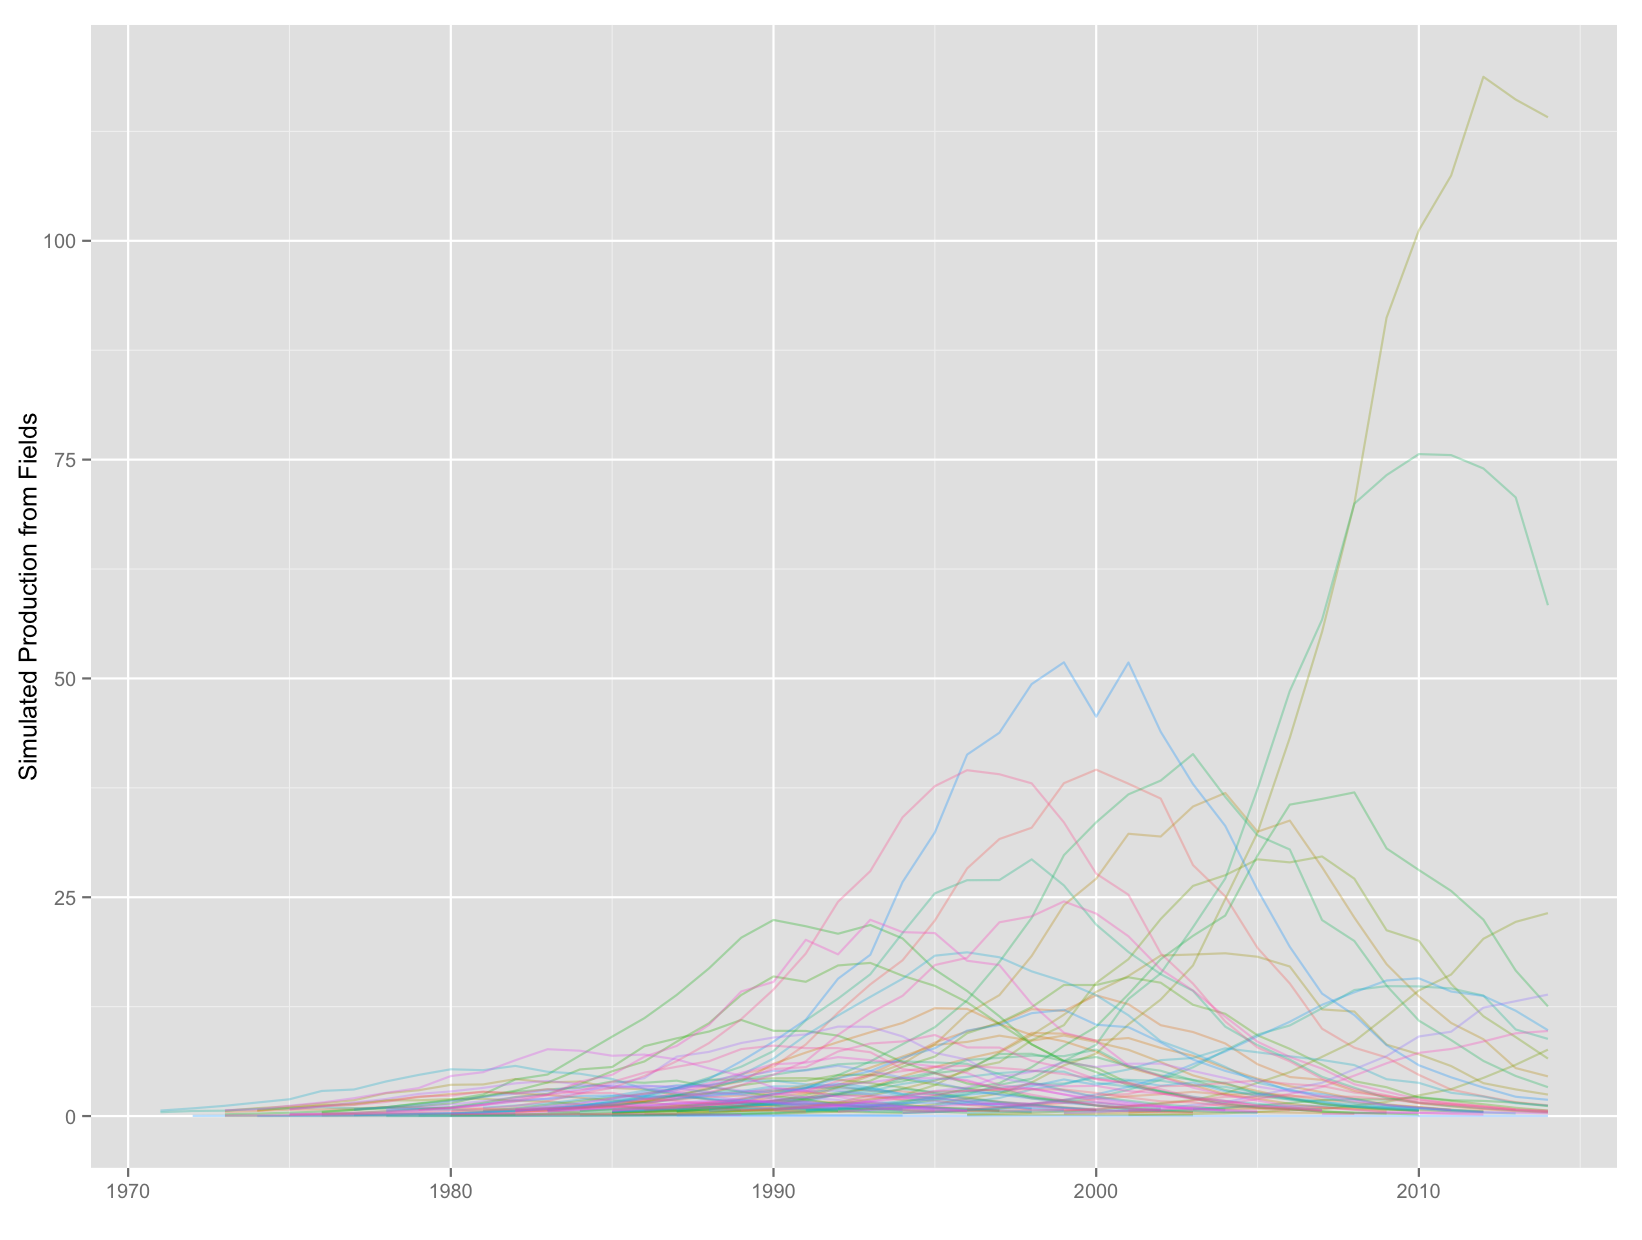
\includegraphics[width=1\textwidth]{figures/simulated_production.png}
	\caption{Simulated production of 77 oil fields}
	\label{simulated_production}	
\end{figure}


\subsection{Estimation of Coefficient}

Within the Monte Carlo function, a regression is run using the gam() function from the package mgcv \citet{wood_generalized_2006}.  This will handle both estimation of linear models or generalized additive models, depending on what formula is passed to the Monte Carlo function.  

\begin{verbatim}
gam_sim<-gam(formula,
	family=gaussian(link=log), weights=size, data=sim_fields)
summary(gam_sim)
\end{verbatim}

Outside of the Monte Carlo function, First I specify a linear regression formula with a 3rd degree polynomial terms to control for the production profile as below.  

\begin{verbatim}
formula_0=formula(prod~time_to_peak + time_to_peak_sq + time_to_peak_cu + 
	peak_to_end + peak_to_end_sq + peak_to_end_cu +size + price)
\end{verbatim}

I then replicate the data 1000 times, letting the $\beta$ term equal zero, that is having no effect of prices on oil production.  The formula used is shown below, where $gam_mc()$ is the Monte Carlo function.  

\begin{verbatim}
gamm_mc_0<-replicate(1000, gam_mc(beta=0, formula=formula_0, use_true_prices=TRUE))
\end{verbatim}

The above line returns 1000 estimates of $\beta$ from the linear regression specification.  Figure \ref{lin_model_price_mc} shows the results in the form of a histogram.

\begin{figure}
	\includegraphics[width=1\textwidth]{figures/lin_model_price_mc.png}
	\caption{Estimated coefficients on price from linear model from Monte Carlo Experiment}
	\label{lin_model_price_mc}	
\end{figure}

As the figure shows, a negative bias in the coefficient is apparent.  The distribution appears double-peaked, with most of the estimates of $\beta$ begin between -.05 and -.01.   

Now consider a specification using a smooth term for the production profile as below.

\begin{verbatim}
formula_1= formula(prod~s(prod_time,size) + price)
\end{verbatim}

Now, the production profile is modeled as a smooth function of production time and size with an additive linear term for price.  Unlike the specification in the body of the article, I do not specify separate smooth terms for pre- and post-peak.  This is simply because I know that the logistic function I used to create the shape of the production profile is symmetric.  

The results of running the Monte Carlo experiment with the specification with the smoothed term are shown in figure \ref{gam_model_price_mc.png}.  Here the estimated coefficient on the price term is centered close to zero, correctly reflecting the true $\beta$.

\begin{figure}
	\includegraphics[width=1\textwidth]{figures/gam_model_price_mc.png}
	\caption{Estimated coefficients on price from GAM model from Monte Carlo Experiment}
	\label{gam_model_price_mc.png}	
\end{figure}

\end{document}